\documentclass{article}
\linespread{1.3}
\usepackage[margin=50pt]{geometry}
\usepackage{amsmath, amsthm, amssymb, amsthm, tikz, fancyhdr, graphicx}
\pagestyle{fancy}
\renewcommand{\headrulewidth}{0pt}
\newcommand{\changefont}{\fontsize{15}{15}\selectfont}

\fancypagestyle{firstpageheader}
{
  \fancyhead[R]{\changefont Michael Huang \\ CFRM 420 \\ Homework 5}
}

\begin{document}

\thispagestyle{firstpageheader}

\section*{1.}
{\Large 

% \begin{verbatim}
%   Text enclosed inside \texttt{verbatim}
%   environment 
%   is printed directly 
%   and all \LaTeX{} commands are ignored.
% \end{verbatim}

% \framebox[1.1\width]{\textbf{answer}}

We can calculate the mean and variance of the distribution which we can use to create a normal distribution according to CLT. Since the yearly log return is the sum of 252 iid daily log returns, we can simply find the 95\% confidence interval by taking 252 multiplied by these 95\% confidence interval bands, giving us \framebox[1.1\width]{\textbf{-0.3991505 to 0.4402316}} according to our seeded sample.

}

\section*{2.}
{\Large

\subsection*{(a)}

We plot this in R, and notice that the symmetry of the distribution tends to shift more towards the middle and a more symmetrical distribution rather than asymmetrical as $n$ increases, while the spread generally gets slightly more refined and tighter as $n$ increases.
\begin{figure}[h!]
  \centering
  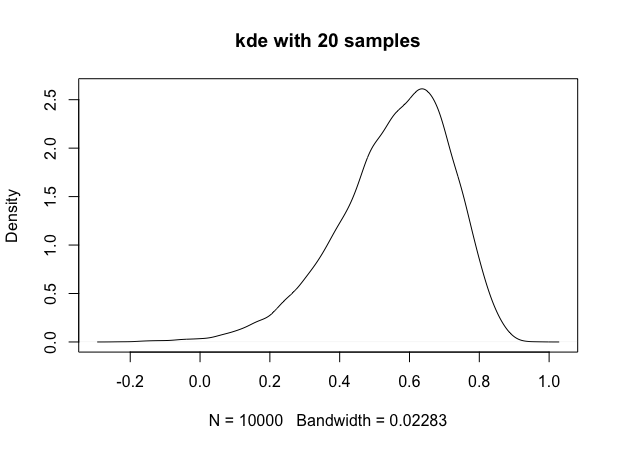
\includegraphics[width=450pt]{hw5_2a_20.png}
\end{figure}
\begin{figure}[t!]
  \centering
  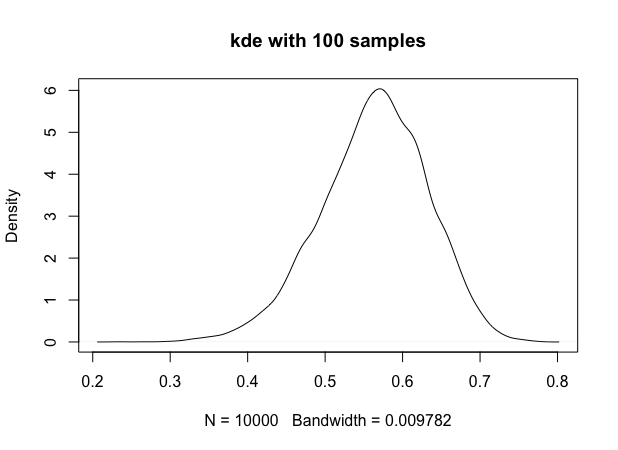
\includegraphics[width=450pt]{hw5_2a_100.png}
\end{figure}
\begin{figure}[t!]
  \centering
  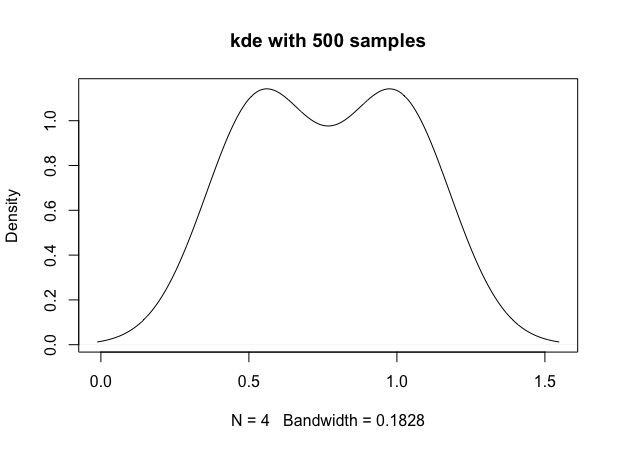
\includegraphics[width=450pt]{hw5_2a_500.png}
\end{figure}
\newpage

\subsection*{(b)}

By definition, we can find each $\text{bias}(\hat{\rho}_n)$ by taking the sum of the means subtracted by the sum of the values: \\
$\text{bias}(\hat{\rho}_{20}) = 
$ -2.00088834390044e-11 \\
$\text{bias}(\hat{\rho}_{100}) = $ 1.45519152283669e-11 \\
$\text{bias}(\hat{\rho}_{500}) = $ 4.54747350886464e-12 \\ \\
By definition, we can find the square root of the variance for each $n$ to estimate $\text{se}(\hat{\rho}_n)$: \\
$\text{se}(\hat{\rho}_{20}) = 0.164072631400487$ \\
$\text{se}(\hat{\rho}_{100}) = 0.0687902431584231$ \\
$\text{se}(\hat{\rho}_{500}) = 0.0306282343447513$

\subsection*{(c)}

As stated, the approximate formulas for large $n$ are $\text{bias}(\hat{\rho}_n) \approx 0$ and $\text{se}(\hat{\rho}_n) \approx \frac{1-\rho^2}{\sqrt{n}} = \frac{1 - (\frac{0.8}{\sqrt{2}})^2}{\sqrt{10000}} = \frac{1 - 0.32}{100} = \frac{0.68}{100} = 0.0068$, since we know that $\rho_{12} = \frac{\sigma_{12}}{\sqrt{\sigma_{11}\sigma_{22}}} = \frac{0.8}{\sqrt{2}}$ and $n = 10000$, as given. \\ \\
Looking at our estimated values, the bias is very close to 0, and only gets better as $n$ increases, while the variance is initially not as close to the actual value but also continues to decrease and get better as $n$ increases.

}

\section*{3.}
{\Large

\subsection*{(a)}

By definition, we know that $\text{bias}(\hat{\theta_1}) = \mathbb{E}[\hat{\theta_1}] - \theta$. We also know that the estimator $\hat{\theta_1}$ is essentially equivalent to doubling the sample mean, or expectation, so we can simplify this expression to be \\
$\text{bias}(\hat{\theta_1}) = \mathbb{E}[\hat{\theta_1}] - \theta = 2 \cdot \mathbb{E}[\theta] - \theta = 2 \cdot \frac{\theta}{2} - \theta = \theta - \theta = 0$, as we aimed to show. \\ \\
By definition, we also know that $\text{se}(\hat{\theta_1}) = \sqrt{\text{Variance}(\hat{\theta_1})}$, and thus we can evaluate this as \\ 
$\text{se}(\hat{\theta_1}) = \sqrt{\text{Variance}(\hat{\theta_1})} \\
= \sqrt{\text{Variance}(\frac{2}{n} \cdot \sum_{i=1}^{n} X_i)} \\
= \sqrt{\frac{4}{n^2} \cdot \text{Variance}(\sum_{i=1}^{n} X_i)} \\
= \sqrt{\frac{4}{n^2} \cdot n \cdot \frac{\theta^2}{12}} $ \hfill Due to the iid nature of $X$, Definition of $\theta$ \\ 
$= \sqrt{\frac{4n\theta^2}{12n^2}} \\
= \sqrt{\frac{\theta^2}{3n}} \\
= \frac{\theta}{\sqrt{3n}}$ \\
which is what we aimed to show.

\subsection*{(b)}

We can find the pdf of $\hat{\theta_2}$ by first taking the derivative of the given cdf: \\ 
$f_{\hat{\theta_2}}(x) = \frac{d}{dx} (\frac{nx}{(n+1)\theta})^n$ \\
$= \frac{d}{dx} (\frac{n^nx^n}{(n+1)^n\theta^n})$ \\
$= \frac{n^{n+1}x^{n-1}}{(n+1)^n\theta^n}$ \\ \\
To find the bias, one component we need to find is the expectation of this pdf. By definition, for the defined uniform distribution, we do this by taking the integral of the pdf multiplied by $x$ over the range $[0, \frac{n+1}{n}\theta]$: \\
$\mathbb{E}(\hat{\theta_2}) $\\
$= \int_{0}^{\frac{n+1}{n}\theta}\frac{n^{n+1}x^{n-1}}{(n+1)^n\theta^n} \cdot x \text{ } dx $ \\
$= \int_{0}^{\frac{n+1}{n}\theta}\frac{n^{n+1}x^n}{(n+1)^n\theta^n} \text{ } dx $ \\ 
$= \frac{n^{n+1}x^{n+1}}{(n+1)^{n+1}\theta^n} |_{x=0}^{\frac{n+1}{n}\theta} $ \\ 
$= \frac{n^{n+1}(\frac{n+1}{n}\theta)^{n+1}}{(n+1)^{n+1}\theta^n} - \frac{n^{n+1}0^{n+1}}{(n+1)^{n+1}\theta^n} $ \\
$= \frac{n^{n+1}(\frac{n+1}{n}\theta)^{n+1}}{(n+1)^{n+1}\theta^n} - 0$ \\ 
$= \frac{n^{n+1}(n+1)^{n+1}\theta^{n+1}}{n^{n+1}(n+1)^{n+1}\theta^n}$ \\ 
$= \theta$ \\ 
Plugging this back into the bias formula: \\
$\text{bias}(\hat{\theta_2}) = \mathbb{E}(\hat{\theta_2}) - \theta = \theta - \theta = 0$ \\ 
as we aimed to show. \\ \\
We can find the standard error by finding $\text{se}(\hat{\theta_2}) = \sqrt{\text{Variance}(\hat{\theta_2})} = \sqrt{\mathbb{E}(\hat{\theta_2}^2) - [\mathbb{E}(\hat{\theta_2})]^2}$ \\
To find the variance, one component we still need to find is $\mathbb{E}(\hat{\theta_2}^2)$, in the same way as we did previously: \\
$\mathbb{E}(\hat{\theta_2}^2)$ \\
$= \int_{0}^{\frac{n+1}{n}\theta}\frac{n^{n+1}x^{n-1}}{(n+1)^n\theta^n} \cdot x \cdot x \text{ } dx $ \\
$= \int_{0}^{\frac{n+1}{n}\theta}\frac{n^{n+1}x^{n+1}}{(n+1)^n\theta^n} \text{ } dx $ \\
$= \frac{n^{n+1}x^{n+2}}{(n+1)^n\theta^n(n+2)} |_{x=0}^{\frac{n+1}{n}\theta} $ \\ 
$= \frac{n^{n+1}(\frac{n+1}{n}\theta)^{n+2}}{(n+1)^n\theta^n(n+2)} - \frac{n^{n+1}0^{n+2}}{(n+1)^n\theta^n(n+2)}$ \\ 
$= \frac{n^{n+1}(\frac{n+1}{n}\theta)^{n+2}}{(n+1)^n\theta^n(n+2)} - 0$ \\ 
$= \frac{(n+1)^{n+2}\theta^{n+2}n^{n+1}}{(n+1)^n\theta^n(n+2)n^{n+2}}$ \\ 
$= \frac{(n+1)^2\theta^2}{(n+2)n}$ \\ 
Plugging this back into the standard error formula: \\
$\text{se}(\hat{\theta_2}) = \sqrt{\mathbb{E}(\hat{\theta_2}^2) - [\mathbb{E}(\hat{\theta_2})]^2} \\
= \sqrt{\mathbb{E}(\hat{\theta_2}^2) - [\mathbb{E}(\hat{\theta_2})]^2}$ \\ 
$= \sqrt{\frac{(n+1)^2\theta^2}{(n+2)n} - \theta^2}$ \\
$= \sqrt{\frac{(n+1)^2\theta^2 - n(n+2)\theta^2}{n(n+2)}}$ \\
$= \sqrt{\frac{(n^2+1+2n)\theta^2 - (n^2+2n)\theta^2}{n(n+2)}}$ \\
$= \sqrt{\frac{\theta^2}{n(n+2)}}$ \\
$= \frac{\theta}{\sqrt{n(n+2)}}$ \\
as we aimed to show.
% 

\subsection*{(c)}

The MSE is defined as $\text{mse}(\hat{\theta}) = \text{bias}(\hat{\theta})^2 + \text{se}(\hat{\theta})^2$, the sum of the bias squared and the standard error squared. Both estimators have bias of 0, so we need only look at the standard error. We can easily see that the denominator of $\hat{\theta_2}$ will increase much more rapidly than that of $\hat{\theta_1}$ as $n$ increases, as the the $n^2$ term in the square root of the denominator of $\hat{\theta_2}$ rather than the $n$ term in the square root of the denominator of $\hat{\theta_1}$ will lead to the overall standard error being much smaller as $n$ increases, which in turn means that the MSE will be much smaller, which means that $\hat{\theta_1}$ will effectively be a better estimator.

}

\end{document}